%*******************************************************************************
%***************************** Finite difference Chapter ***********************
%*******************************************************************************

\chapter{The Finite Difference Method}
\label{ch:FDM}
\vskip 1em
\dictum[Bertrand Russel]{%
	All exact science is dominated by the idea of approximation. When a man tells you that he knows the exact truth about anything, you are safe in infering that he is an inexact man.. }%
\vskip 1em
\dictum[John von Neumann]{%
	Truth … is much too complicated to allow anything but approximations. }%
\vskip 1em

\lettrine[lines=3,lhang=0.33,lraise=0,loversize=0.15]{M}{ost} of the Partial Differential Equations (PDE) arising from formulation of physical problems are very hard to solve analytically, requiring approximate numerical solution.
An important part of handling and solving PDEs is to be able to use local,accurate and stable algebraic expression as an approximation of the derivatives appearing in the equations retaining, at the same time, most of the global and continuous information of the original formulation.
During the last half century several methods approximation methods have been developed and studied, such as the finite volume (FV), finite element (FE), and finite difference (FD) methods (FDM), each with specific approaches to discretization. 
This chapter briefly describes the concept of differential equation and introduces their numerical solution using the Finite Difference Method. For a rigorous and complete descritpion of the topic of this chapter please refer to \cite{cita qui un paio di lavori}.

\subsection{Differential Equation}
A differential equation is an equation where the unknown is a function itself and where derivatives ot the unknown appears in the equation \cite{Larsoon:2004} \cite{Mcowen:2002}. Differential Equations can be divided into two main classes:

\begin{description}
\item[Ordinary Differential Equation (ODE)] where the unknown function contains only derivatives with the respect of a single variable. As example of ODE is the following
\[
  \frac{d T}{d x} = \alpha T(x) +b
\] where $a$ and $b$ are some constant.

\item [Partial Differential Equations (PDE)] which is an extremely large and rich of functions class each of them with a different behavior and properties. Examples of classes in of this kind of differential equations are parabolic, elliptic or hyperbolic equations. PDEs search for a multidimensional function of several variables, and this means that partial derivatives may now appears in the equation. 
Examples of famous PDEs are:
   \begin{descritpion}
     \item [Transport Equation:] \hfil \\
     \begin{equation}
		\frac{\partial T}{\partial t} + \frac{\partial T}{\partial x} =0
     \end{equation}
     \item [diffusion equation:]\hfil \\ 
     \begin{equation}
     	\frac{\partial T}{\partial t} - \frac{\partial^2 T}{\partial x^2}=0
     \end{equation} 
     \item [1D wave equation:]\hfil \\  
     	\begin{equation}
     	\frac{\partial^2 T}{\partial t^2} -\frac{\partial^2 T}{\partial x^2}=0
     	\end{equation}
     \item [Laplace's equation:]\hfil \\  
     	\begin{equation}
     	\frac{\partial^2 T}{\partial x^2} + \frac{\partial^2 T}{\partial y^2}=0
     	\end{equation}
     \item [Heat equation:]\hfil \\  
     	\begin{equation}
     	\frac{\partial T}{\partial t} - \kappa \frac{\partial^2 T}{\partial x^2}=0
     	\label{eq:heat_equation}
     	\end{equation}
   \end{descritpion}
\end{description}
Note that there is a missing piece that would allow all these equation to be solved unequivocally. The initial condition and/or boundary. For example, regarding the 1D wave equation, what is the reflection coefficient at the ends of the string? 
Initial condition must be provided whenever the differential equation is time dependent. Boundary conditions must be specified whenever spacial dependency occurs. Boundary conditions specify the behavior of the equation at the boundary of the domain $\partial \Gamma$ (which has to be compact). Most common boundary conditions are of two kind:
\begin{description}
	\item [Dirichlet:] \hfil \\ in which the values of the functions at $\partial \Gamma$ are hard-coded, i.e. $T(\partial \Gamma)$  is known.
	
	\item [Neumann:] specifies values of the derivatives at $\partial \Gamma$.
	
\end{description} 
Other kind of boundary conditions are possible, such as for instance the Robin's boundary conditions which is a mix of Dirichlet and Neumann ones. See Figure \ref{fig:heat2d_bc} for an example of Dirichlet boundary conditions for the equation \ref{eq:heat_equation}.

    \begin{center}
	\begin{figure}
    	\begin{tikzpicture}
    	\node[anchor=south west,inner sep=0] at (0,0) {\includegraphics[scale=0.3]{./images/CA_FDM/heat2d_bc}};
    	\draw<1>[red,ultra thick,rounded corners] (1.9,0.94) rectangle (\textheight-14cm,1.3);
    	\draw<1>[red,ultra thick,rounded corners] (1.9,8.94) rectangle (\textheight-14cm,8.6);
    	
    	\draw<1>[red,ultra thick,rounded corners] (1.9,0.8) rectangle (2.3,\textheight-14.7cm);
    	\draw<1>[red,ultra thick,rounded corners] (9.5,0.8) rectangle (9.9,\textheight-14.7cm);
    %	\draw<2>[red,ultra thick,rounded corners] (5.7,4.1) rectangle (7.5,4.9);
   
    	\end{tikzpicture}
    	 \label{fig:heat2d_bc}
    	\caption[Heat Equation Boundary Conditions]{Heat Equation (see Equation \ref{eq:heat_equation}) Dirichlet Boundary Conditions. The perimeter of the square domain (highlighted in red) has fixed temperature, i.e. the solution $T$ is known at the boundary. In particular, $T(x,0)=T(0,y)=0$, $T(1,x)=3$ and $T(1,y)=2$ where $0\leq x,y\leq 1$. }\label{fig:heat2d_bc}
	\end{figure}
\end{center} 

%------------------Finite difference Formulas-------------------------------
    \section{Finite Difference Method}
The finite difference approximation for derivatives is one of the simplest oldest method to solve differential equations numerically. It was used since 1768 by \textit{L. Euler} to solve one dimensional problems and extended by \textit{C. Runge} to two dimension in 1910. Since the advent of computers in 1950, FDM  popularity skyrocketed also thanks to the theoretical results that have been obtained regarding stability, convergence and other of its properties during the last five decades.

The general idea behind FDM is that the differential operator is approximated by replacing the derivatives using difference quotients. The differential operator is approximated constituting the field equation locally, among a number of finite function values. Therefore, the space and time domain are \textit{partitioned} in a grid like fashion in order to store the local field quantities, and approximated solutions are computed only for those discrete grid points. The numerical solution is known only at a finite number of points in the physical domain. 
Difference quotients are linear combination of function values at neighboring grid points. The number of different points appearing in the quotient directly dictates the order ot the differential operator.
We can always assume rectangular grid since we can always  specify boundary conditions for the grid points such that they mimic the real shape of the boundary at hand, (see Figure \ref{fig:gridcustomshape}).
The values of such points that lie on
A refinement on the treatment of complex geometries and curvilinear boundaries is compute the value of such points that lie on the boundary as a linear interpolation of neighboring boundary grid points as shown in Figure \ref{fig:gridcustom_shape2} and Equation \ref{eq:interpolateboundary}.

\begin{equation}
   T(R) = \frac{T_4(h-\delta) + T_0 \delta}{h} = g_0(R)
   \label{eq:interpolateboundary}
\end{equation}
where $g_0$ specifies the values at the boundaries.
\begin{figure}
	\minipage{0.44\textwidth}
	\begin{subfigure}{1.0\textwidth}
		\includegraphics[width=\linewidth]{./images/CA_FDM/grid_custom_shape}
		\label{fig:gridcustomshape}
		\caption{Discretization of a curvilinear domain.}
	\end{subfigure}		
	\endminipage\hfill
	\minipage{0.53\textwidth}
	\begin{subfigure}{1.0\textwidth}
		\includegraphics[width=\linewidth]{./images/CA_FDM/gridcustom_shape2}
		\label{fig:gridcustom_shape2}
		\caption{Interpolation of boundary values on a non rectangular geometry domain.}
	\end{subfigure}
	\endminipage\hfill
\end{figure}

Figure \ref{fig:schematic_repr_fdm} is a schematic representation of how FDM are used to obtain a numerical solution. The continuous differential operators and the domain are discretized. The approximation is computed solving the difference formulas on grid points using.

   

\begin{figure}[b]
    \centering
  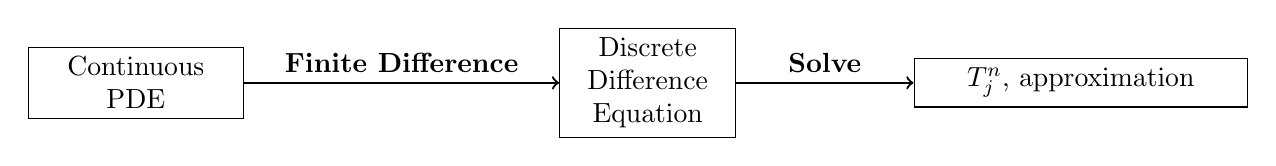
\begin{tikzpicture}

    \node[draw, text centered,text width=2.5cm] (1) at (0,0) {Continuous PDE};
    \node[draw, text centered,text width=2cm] (2) at (6.5,0) {Discrete Difference Equation};
    \node[draw, text centered,text width=4cm] (3) at (12,0) {$T_j^n$, approximation};

\draw[thick,->] (1) -- (2) node[midway,sloped,above,rotate=0] {\textbf{Finite Difference}};
\draw[thick,->] (2) -- (3) node[midway,sloped,above,rotate=0] {\textbf{Solve}};
\end{tikzpicture}
    \caption{Relationship between continuous and discrete problems.}
    \label{fig:schematic_repr_fdm}
\end{figure}
    
    The error, between the numerical solution and the exact solution is determined by the difference formula utilized and is commonly refeered as \textit{truncation}\footnote{The term truncation comes from the fact that a finite difference quotient is a truncation of the Taylor expansion.} or \textit{discretization} error.  Increasing the resoution of the grid increases the accuracy of the numerical solution since the error associated with the finite difference formulas directly depends on the distance between grid points.
    
        
    Depending on how the derivatives are approximated, explicit or implicit FDM schemes are
    obtained. When forward difference formulas are considered, the
    resulting difference equation is generally expressed in terms of
    an explicit recurrence formula, while backward difference formulas
    generally lead to implicit recurrence formulas involving unknown
    values, and therefore require the solution of a linear system to
    obtain the new state of the system at each grid point.
    
    
\subsection{Finite Difference Formulas}
Differential operator appearing in a PDE problem can be approximated at a given point by a difference formula which is a linear function of its neighboring grid points. There is a number of ways of defining and deriving a finite difference formula but some of them are more widely and commonly used then others. The rest of this section shows how  these common formulas are derived along with their basic properties. 

For the sake of simplicity the formulas are refereed to a one-dimensional space and time domain since the generalization to several dimensions is obvious.
Both space and time domain are partitioned into a finite discrete mesh as follows:    
 \begin{equation}
    		t_n = n\Delta t, \: n = 0,1,\ldots,L,\; \Delta t= \frac{1}{L}
    \end{equation}
    \begin{equation}
    		x_j = j\Delta x, \: j = 0,1,\ldots,M,\;\Delta x = \frac{1}{M}
    \end{equation}

For the rest of the chapter, it can be assumed that grid points are identifies by two indices (see Figure \ref{fig:fdmheatequationstencil}) and $T_j^n$ is the value the function at time $n$ at grid point $j$.

\subsection{Forward Scheme}
    Probably the most common FD formula can be derived from Taylor's expansion of $T^n_{j+1}$ in terms of $T^n_{j}$ and its derivatives as:
    
    \begin{equation}
    T^n_{j+1} = T^n_{j} +
    \frac{\partial T}{\partial x}\bigg\rvert^n_j \Delta x +
    \frac{1}{2!}  \frac{\partial^2 T}{\partial x^2}\bigg\rvert_j \Delta x^2 + \ldots + 
     \frac{1}{k!}  \frac{\partial^k T}{\partial x^k}\bigg\rvert_j \Delta x^k + \ldots
     \label{eq:taylorexp1}
    \end{equation}
    
    If series is truncated after the second term ($k=1$) and solving for $\frac{\partial T}{\partial x}$ the following is obtained:
    
    \begin{equation}
    \frac{\partial T(t,x)}{\partial x}  = \frac{T^n_{j+1} - T^n_{j}}{\Delta x} + \mathcal{O}(\Delta x)
    \label{eq:fdmforward}
    \end{equation}
    
    Equation \ref{eq:fdmforward} is called fist \textbf{forward} finite difference approximation. Other approximations are possible and are easily obtainable by expanding different points of the grids and using more points from the expansion.
    
  \subsection{Backward Scheme}  
    \textbf{Backward} finite difference quotient can be obtained from the Taylor's expansions of    
        \begin{equation}
    T^n_{j-1} = T^n_{j} - 
    \frac{\partial T}{\partial x}\bigg\rvert_j \Delta x +
    \frac{1}{2!}  \frac{\partial^2 T}{\partial x^2}\bigg\rvert_j \Delta x^2 + \ldots + 
     \frac{1}{k!}  \frac{\partial^k T}{\partial x^k}\bigg\rvert_j \Delta x^k + \ldots
     \label{eq:taylorexp2}
    \end{equation}
    
    which can be rearranged in the following manner
        \begin{equation}
    \frac{\partial T}{\partial x}\bigg\rvert_j  = \frac{T^n_{j} - T^n_{j-1}}{\Delta x} + \mathcal{O}(\Delta x)
    \label{eq:fdmfbackward}
    \end{equation}
    
   The same approach can be used to derive approximation for higher order derivatives.
   For example equation \ref{eq:fdmcentral}, known called \textbf{central difference formula}, is an approximation for the second order derivative and can be obtained retaining the firsts four terms in both equations \ref{eq:taylorexp1} and \ref{eq:taylorexp2} and adding the resulting expression:
   
    \begin{equation}
		\frac{\partial^2 T}{\partial x^2}\bigg\rvert_j = \frac{T^n_{j+1}- 2T^n_{j} + T^n_{j-1}}{\Delta x^2} + \mathcal{O}(\Delta x^2)
		\label{eq:fdmcentral}
    \end{equation}
    
    Figure \ref{fig:geometrical_intepretation} show how finite difference formulas can be interpreted geometrically.
\begin{figure}
	\centering
	\includegraphics[width=0.85\textwidth]{./images/CA_FDM/geometrical_interpretation_fd}
	\label{fig:geometrical_intepretation}
	\caption{Explicit FDM discretization for the 1D heat conduction problem}\label{torus}
\end{figure} 
    
Note that this approach in deriving FD formulas can be generalized in order to obtain FD approximation for derivatives of any order.

 \subsection{Mixed Derivatives}

Mixed derivatives con also be approximated using FDM, e.g. for two dimensions by means of the following property of mixed derivatives:
\begin{equation}
\frac{\partial ^2 T}{\partial x \partial y} = \frac{\partial}{\partial x} \Bigg{(}\frac{\partial T}{\partial y}\Bigg{)} = \frac{\partial}{\partial y} \Bigg{(}\frac{\partial T}{\partial x}\Bigg{)}\\
\end{equation}
and considering the following approximations:
\begin{equation}
\begin{cases}
&\frac{\partial ^2 T}{\partial x \partial y} = 
\frac{\bigl(\frac{\partial T}{ \partial y}\bigr)_{i+1,j}\, - \,
	\bigl(\frac{\partial T}{ \partial y}\bigr)_{i-1,j}
}{2\Delta x} +\mathcal{O}(\Delta x)^2 \\
&\bigl(\frac{\partial T}{\partial y}\bigr)_{i+1,j} = \frac{T_{i+1,j+1} -T_{i+1,j-1}}{2\Delta y}+\mathcal{O}(\Delta y)^2 \\
&\bigl(\frac{\partial T}{\partial y}\bigr)_{i-1,j} = \frac{T_{i-1,j+1} -T_{i-1,j-1}}{2\Delta y}+\mathcal{O}(\Delta y)^2 \\
\end{cases}
\end{equation}
A second order 2 variables finite difference approximation for the mixed derivative is the following:

\begin{equation}
\Bigg{(}\frac{\partial ^2 T}{\partial x \partial y}\Bigg{)}_{i,j}= \frac{T_{i+1,j+1} -T_{i+1,j-1} - T_{i-1,j+1} -T_{i-1,j-1}}{4\Delta x \Detla y} +\mathcal{O}((\Delta x)^2,(\Delta y)^2)
\end{equation}

Extending the former method to higher dimensional mixed derivatives is straightforward.
    %------------------HEAT Equation-------------------------------
    \section{Heat Equation}
        As an example a simple FDM scheme for an initial-boundary condition problem for the heat conduction problem is derived. 
    
\begin{equation}
    \frac{\partial T(t,x)}{\partial t}= \kappa\frac{\partial^2
      T(t,x)}{\partial x^2}
      \label{eq:heatconduction}
\end{equation}
 
    where $0 \leq t \leq L$ and $0 \leq x \leq
    M$. 
 In order to construct a FD approximation for equation \ref{eq:heatconduction} 
 
 \begin{figure}[b]
 	\centering
 	\includegraphics[scale=0.5]{./images/CA_FDM/heatstencil}
 	\label{fig:fdmheatequationstencil}
 	\caption{Explicit FDM discretization for the 1D heat conduction problem}\label{torus}
 \end{figure}   
 
 \begin{enumerate}
 
 \item Discretize the domain into a finite regular mesh where each point $x_j$ is identified with a unique index $j$.
    
 \item  First and second order derivative appearing in \ref{eq:heatconduction} are substituted by forward and central difference formulas, respectively, leading to Equation \ref{eq:discretizedheatequation} (see Figure  \ref{fig:fdmheatequationstencil}):
 
 \begin{equation}
  \frac{T^{n+1}_{j} - T^n_{j}}{\Delta t} = \kappa \frac{T^n_{j+1}- 2T^n_{j} + T^n_{j-1}}{\Delta x^2}
 \label{eq:discretizedheatequation}
 \end{equation}
 
 \item Equation \ref{eq:heatconduction} is evaluated at grid point $(n\Delta t, j \Delta x)$ 
    
\end{enumerate}    
    

    
\begin{figure}
\centering
\includegraphics[width=0.8\textwidth]{./images/CA_FDM/fdmgrid}
\caption{1D heat equation FDM grid space and time partitioning.}\label{torus}
\end{figure}

Solution to equation \ref{eq:heatconduction} using the discretization \ref{eq:discretizedheatequation} is called \textit{forward time, centered space or FTCS} approximation and requires the specification of initial conditions at $t=0$ and boundary condition at $x=0$ and $x=M$ (see Figure \ref{fig:heat2d_bc}).

It can be shown that in order to the solution to be stable $\Delta t$ must not be too large and in particular the following condition must hold to ensure a stable solution \cite{isaacson:1994,anderson:1994,crank:1996}:
\[ 
 r= k \frac{\Delta t}{\Delta x^2}< \frac{1}{2}
\]

This scheme is also called explicit because values the the next time are explicitly computable from the values at the current time as it is shown in the equation \ref{eq:discretizedheatequation1}.
 \begin{equation}
  T^{n+1}_{j} = T^n_{j} + \frac{k \Delta t}{\Delta x^2} (T^n_{j+1}+T^n_{j-1}-2T^n_{j})
 \label{eq:discretizedheatequation1}
 \end{equation}

%%backward heat equation
When the backward difference formula is used for approximating the time derivative the following approximation is obtained

 \begin{equation}
  \frac{T^{n}_{j} - T^{n-1}_{}}{\Delta x} = k \frac{T^n_{j+1}- 2T^n_{j} + T^n_{j-1}}{\Delta x^2}
 \label{eq:discretizedheatequation_implicit}
 \end{equation}
 This stepping scheme is called implicit because values at time $n$ are given implicitly as can be seen if equation \ref{eq:discretizedheatequation_implicit} is rearranged to obtain the following: 
 \begin{equation}
T^n_{j} - \frac{k \Delta t}{\Delta x^2} (T^n_{j+1}+T^n_{j-1}-2T^n_{j}) =   T^{n-1}_{j}
 \label{eq:discretizedheatequation1}
 \end{equation}
 In order to obtain values of T at time $n$ a system of non trivial algebraic equation has to be solved. 
 It can be rewritten in matrix form yielding to a tridiagonal matrix (see Section \ref{sec:tridiagonal})

\begin{equation}
\begin{tikzpicture}[baseline=(current bounding box.center)]
\matrix (m) [matrix of math nodes,nodes in empty cells,right delimiter={]},left delimiter={[} ]{
  (1+2\lambda)  & -\lambda     &          &  &  &  & &  \\
  -\lambda      & (1+2\lambda) & -\lambda &  &  &  & & \\
  &             &              &          &  &  &  & & \\
  &             &              &          &  &  &  & & \\
  &             &              &          &  &           &             &           \\
  &             &              &             &    -\lambda &(1+2\lambda) & -\lambda \\
  &             &              &          &  &           &  -\lambda   &(1+2\lambda) \\
} ;
\draw[line width=1pt,line cap=round,loosely dotted] (m-2-2)-- (m-6-6);
\draw[line width=1pt,line cap=round,loosely dotted] (m-2-3)-- (m-6-7);
\draw[line width=1pt,line cap=round,loosely dotted] (m-2-1)-- (m-6-5);
\end{tikzpicture}
\begin{tikzpicture}[baseline=(current bounding box.center)]
\matrix (m) [matrix of math nodes,nodes in empty cells,right delimiter={]},left delimiter={[} ]{
	 T_1^n  &   \\
	T_2^n   &  \\
			&\\
			&\\
			&\\
			&\\
			&\\
			&\\
	T_M^{n} \\
} ;
\draw[line width=1pt,line cap=round,loosely dotted] (m-3-1)-- (m-8-1);
\end{tikzpicture}
=
\begin{tikzpicture}[baseline=(current bounding box.center)]
\matrix (m) [matrix of math nodes,nodes in empty cells,right delimiter={]},left delimiter={[} ]{
	T_1^{n-1}  &   \\
	T_2^{n-1}   &  \\
	&\\
	&\\
	&\\
	&\\
	&\\
	&\\
	T_M^{n-1} \\
} ;
\draw[line width=1pt,line cap=round,loosely dotted] (m-3-1)-- (m-8-1);
\end{tikzpicture}
\label{eq:eqq1}
\\ \eqname{asdfsdf}
\end{equation}
  where $\lambda = \frac{k\Delta t}{\Delta x^2}$ for which an efficient algorithms exist, Thomas's algorithm \cite{Datta:2010,Higham:2002}, which solves it in ${\Theta}(n)$ where $n$ is the number of unknowns.
 


        
    %%XCA and finite difference method-----------------------------------
\section[Solving FDM with XCA]{Solving Finite Difference Problems FDM with Extended Cellular Automata}
    XCA can be employed for both explicit and implicit schemes to
    represent FDM models in formal terms. In fact, in case of an
    explicit scheme, the computational domain can be represented by
    means of the $R$ cellular space and the coordinates of the grid
    points involved in the recurrence formula defined by means of the
    $X$ neighbourhood relationship. Moreover, the values of involved
    variables can be represented in terms of substates and the
    explicit recurrence formula easily expressed in terms of
    elementary processes. Instead, while dealing with a linear system
    resulting from an implicit FDM scheme, a steering function can be
    employed instead of elementary processes, together with an
    external linear algebra solver.

    It is worth to recall that physically-based models laying on a XCA
    direct discrete approach (i.e., not going through the
    discretization of differential equations) can lead to the same
    discrete formulations achieved with the FDM, making these latter
    formulations a specific case of the general XCA
    approach. \cite{Mendicino:2006} proved that
    their direct discrete formulation of the Darcy equation for
    modelling unsaturated flow in a three-dimensional cubic cell
    system is similar to the one achieved using an explicit FDM or
    finite volume scheme. However, the same discrete governing
    equation system would allow a greater level of convergence with
    respect to traditional methods if an irregular mesh is used
    and a not linear (e.g., quadratic) interpolation of the hydraulic
    head on the cells is adopted (e.g., Tonti proved it for the Finite
    Element Method \cite{Tonti2001237}). This is a potential of the XCA
    approach that will be exploited in future versions of OpenCAL,
    where also non-regular grids will be allowed.






